\scanpage{62}
% archive foliation: 61
On trouve
\[
\operatorname{Aut}^0(C,a)\simeq\prod_{x\in C_0\setminus\{a\}}\deleted{\unsure{G_x}}\pi_x
\]
\figure{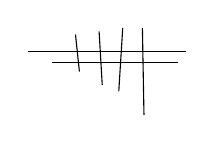
\begin{tikzpicture}[x=1cm,y=1cm]
\draw (0,0)--(2,0) (.3,-.14)--(1.9,-.14);
\draw (.6,.22)--(.65,-.25) (.9,.26)--(.94,-.42) (1.2,.3)--(1.15,-.5) (1.45,.3)--(1.47,-.8);
\end{tikzpicture}}
\deleted{Soit $K$ un graphe}

Soit $I$ un ensemble muni d'une structure polygonale d'ordre $n\geq2$ \deleted{i.e. \unsure{$\Delta_0$}} [pour $n=\unsure{2}$, il faut se donner l'ens. \inserted{de cardinal $2$} des arêtes $\unsure{I^*|I^+}$, \deleted{de} ou ce qui revient au \unsure{$=$|m\textsuperscript{e}}, $\Omega(\Pi)\simeq I\unsure{\wedge|\times}I^*\ldots$ \deleted{cardinal $2$, et}], $\unsure{\mathbb D|D}\ (\simeq\unsure{\mathbb D|D}_n)$ le gr. des autom. de $I$.

Soit $K=K(I)$ le graphe donné par
\diagram{\ensuremath{\begin{array}{ll}
\uline{\text{Sommets}}:&\unsure{\operatorname{Ob}(\Pi)|\Omega(\Pi)}=C_0=\{o,o'\}\\[4pt]
\uline{\text{arêtes}}&\unsure{I^*|I}\quad(\text{indexation }(l_i)_{i\in I})
\end{array}}}
\deleted{\unsure{Toute arête est incidente}}

Incidence : $\unsure{C_0|G_0}\times I$ (\unsure{tte|tt} arête incidente à \unsure{ts|tt} sommets)

\inserted{$G$ opère sur $K(I)$, et on a aussi l'``\uuline{involution}'' $\tau$ qui est l'identité sur $I$, et échange $o,o'$, commutant à $G$.}

\figure{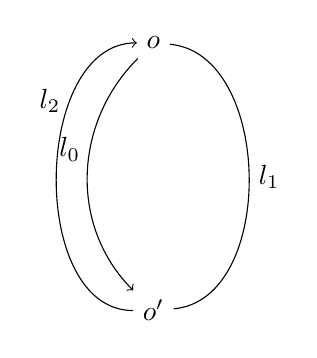
\begin{tikzpicture}[x=1cm,y=1cm]
\node (o) at (0,1.7) {$o$};\node (p) at (0,-1.7) {$o'$};
\draw[->] (p) to[out=180,in=180] node[left,pos=.7] {$l_2$} (o);
\draw[->] (o) to[out=-135,in=135] node[left,pos=.4] {$l_0$} (p);
\draw (o) to[out=-5,in=5] node[right] {$l_1$} (p);
\end{tikzpicture}}
Soit $C(I)$ le groupoïde fondamental de $K(I)$. \deleted{le gr.} $G$ y opère par automorphismes, en opérant transitivement sur $C_0=\{o,o'\}$.

On va regarder le \deleted{commutant}\inserted{normalisateur de $G$} dans
